% --------------------------------------------------------------------------- %
% --------------------------------------------------------------------------- %
\chapter{Extending the All-Hadronic Search}
\label{ch:soft}

The results presented in this analysis thus far exclude significant amounts of SUSY parameter phase space compared to previous searches for similar signatures. However, the spectrum of SUSY models that might be realized in nature is wide and varied. As the LHC continues to deliver an increasing amount of collision data, the ability to probe increasing rare and more subtle signatures increases. 

In this final section we discuss extensions to the \mttwo analysis that modify the search to target additional SUSY models, in particular those which may produces very low-\pt leptons in the final state, otherwise known as {\it soft leptons}. By requiring a lepton in the final state, the previously irreducible invisible Z background of the all-hadronic analysis is greatly suppressed, and in principle one might hope to probe additional phase space for new physics.

\section{Natural Supersymmetry and EWKinos}
\label{sec:natural}

There are a multitude of supersymmetric models which solve some of the theoretical issues of the SM, namely the hierarchy problem discussed in section \ref{sec:smIssues}. However, given the vast parameter of SUSY phase space which might satisfy physical constraints, it is sometimes considered theoretically unfavorable for a particular model to accomodate physical phenomena at the expense of a theoretical explanation, instead relying on the ``fine-tuning'' of physical parameters to remain consistent with observations in nature. The property of a theoretical model that consistently explain observed phenomena with minimal tuning is often referred to as its {\it naturalness}, and can be quantified as a the likeliness for measured observables to be contained in some subset of the total parameter space such that the model satisfies experimental constraints.

A SUSY model that solves some of the fine-tuning problems present in the SM without introducing additional fine-tuning problems of its own is an example of {\it natural supersymmetry}, and is theoretically appealing as an elegant solution to the would-be fine-tuning issues in the SM \cite{Casas:2014eca}. Such natural models often share similar characteristics, including a relative mixing of the supersymmetric partners of the Higgs and electroweak gauge bosons (EWKinos) into mass eigenstates with a highly-degenerate spectrum. Charged EWKinos (\chipm) can decay into neutral EWKinos or the lightest supersymmetric particle (\chiz) in cascades with leptons in the final state. In compressed mass spectra where the mass difference between the charged and neutral EWKinos is small, the outgoing leptons will be soft, and searches targeting soft leptons in the final state can be a useful tool in searches for natural SUSY.

\section{The Soft Lepton Search}
\label{sec:softlep}

A preliminary search extending the all-hadronic analysis was conducted on 2.3\fbinv of data collected by the CMS detector through 2015 \cite{CMS-PAS-SUS-16-011}. The results of this preliminary analysis are presented here and interpreted in the context of two simplified SUSY models with compressed spectra.

\subsection{Event Selection}
\label{subsec:softevents}
The soft lepton search defines a baseline selection similar to that used in the \mttwo analysis, with the notable exception of requiring a soft electron (muon) with $5 < \pt < 20\GeV$ in the barrel region, $|\eta| <$ 1.4442 (1.479). Similar \MET triggers are used, with a minimum \MET requirement of 200\GeV to saturate the trigger efficiency. Identical \dphilong and \htovermet requirements are used to protect against \MET mismeasurements, and
to reject dilepton events the same lepton vetoes are applied to additional leptons in the event. There is an additional requirement on transverse mass of the soft leptons such that $\mt > 20\GeV$, in order to reduce the background contribution from $Z\rightarrow\tau\tau$ events. Events must contain at least 1 jet and a minimum of $\HT > 200\GeV$ of hadronic activity.

Following the baseline selection above, events are further categorized into topological regions using the \HT, \MET, and \nj content, as well as the number of b-tags \nbsoft and \nbhard, where a b-jet is considered soft if $20 < \pt < 50\GeV$, and hard if $\pt > 50\GeV$. There are three ``tail'' regions corresponding to different kinematic variables:
\begin{itemize}
	\item \nb (soft or hard) $\geq 3$
	\item $\MET > 500\GeV$ and $\nb \leq 3$
	\item $\HT > 1000\GeV$, $\nb \leq 3$, and $\MET < 500\GeV$
\end{itemize}
The remaining phase space is divided into topological regions as follows:
\begin{itemize}
	\item \MET : [200,300], [300,500] \GeV. These are merged in the monojet regions with b-tags.
	\item \nb : There are four \nb regions, \nb = 0, \nbsoft = [1,2] (with \nbhard = 0), and \nbhard = [1,2], respectively referred to as the 0b, soft b, and hard b regions.
	\item \nj : In regions with no b-tags, events are binned in regions with 1, 2-3, 4-5, or $\geq$6 jets. In regions with one or more b-tags, events are binned in regions with 1, 2-3, or $\geq$4 jets.
\end{itemize}
Finally, each topological region is subdivided into three bins of \mt: [20,90], [90,120], and $\geq$120\GeV. In total, there are 21 topological regions each subdivided into 3 \mt bins.

\subsection{Backgrounds}
\label{subsec:softbkgs}
The background for the soft lepton analysis can be categorized into three separate sources:
\begin{itemize}
	\item {\it Single Lepton}: real SM processes can generate events with a single lepton in the final state. Typically such events contain a single leptonically decaying W boson (from either W production, top quark production, or other rare processes), and also generate significant missing energy due to the neutrino associated with the W decay.
	\item {\it Dilepton}: SM events with two (or more) leptons in the final state can be mischategorized when other leptons are misidentified or not reconstructed. Typically such events are due to two leptonically decaying W bosons (from either \ttbar or diboson production), where one of the W-associated leptons is not found. Because there are usually two neutrinos contributing to the \MET vector, \mt is less effective in discriminating against this background.
	\item {\it Fake Lepton}: events without any lepton in the final state (such as QCD multijet production of \znunu) can enter the signal region if a jet is misidentified as a lepton or a non-prompt lepton passes the lepton selection. This background is highly suppressed and typically negligible in all but some high-\mt regions.
\end{itemize}

%single lepton estimate
\subsection{Single Lepton Estimate}
\label{subsec:soft1Lestimate}
The single lepton background is primarily due to highly-asymmetric W decays where the neutrino carries a large fraction of the W momentum, resulting in a large \MET and a soft lepton. These events are greatly suppressed by sampling the \mt distribution as values greater than the W mass, and is estimated in all signal regions using a control region with an inverted asymmetry. A single high-\pt control region is created by selecting events with a single lepton above the corresponding \MET threshold in a given signal region (\pt $\geq$ 200, 300, or 500 \GeV), with an maximum threshold on the missing energy $\MET <60\GeV$ so that the W momentum distribution is kinematically similar to that in the signal regions. The number of control region events in a given topological region ($N^{\text{CR1L}}$) is multiplied by the ratio of SR-to-CR events as calculated in simulation ($R_{\text{MC}}^{\text{SR/CR1L}}$) for the region, and extrapolated into bins of \mt based on simulation ($k_{\text{MC}}(\mt)$) as described in equation \ref{eq:soft1Lestimate}. The extrapolation in bins of \mt is necessary not only to preserve statistics but because the shape of the \mt distribution in each control region is very different from the signal region distribution, due to the low-\MET requirement in the control region where resolution effects cause a significant smearing in the \mt shape.
\begin{equation}
	N_{1l}^{\text{SR}} = N^{\text{CR1L}} \cdot R_{\text{MC}}^{\text{SR/CR1L}} \cdot k_{\text{MC}}(\mt)
	\label{eq:soft1Lestimate}
\end{equation}

The uncertainties associated with the single lepton estimate account for statistical fluctuations in data and simulation, as well as possible sources of systematic error in simulation propagated to the quantities measured in MC. The polarization modeling is studied in an inclusive W sample and found to be well modeled by simulation, and additional studies reweighting simulation based on W polarization result in an uncertainty of 10-20\% on the transfer factor $R_{\text{MC}}^{\text{SR/CR1L}}$. Additional uncertainties due to the relative fraction of top and W events, renormalization and factorization scales, lepton efficiency, b-tagging efficiency, jet energy corrections, and uncertainty on top momentum are propagated through simulation, with varying effects between 1-10\%. In addition, multiple uncertainties associated with \mt modeling in simulation are studied, with effects due to W-top fraction and \MET resolution yielding uncertainties ranging between 5-30\% in \mt shape, depending on the relative fraction of top events in a given bin.

%dilepton estimate
\subsection{Dilepton Estimate}
\label{subsec:soft2Lestimate}
Backgrounds due to dilepton events where one lepton is not found are estimated using a control region instead requiring two leptons, replacing the second-lepton veto with a tight requirement for a second, high-\pt lepton. To suppress the contribution from events with fake leptons, the second lepton is required to have a minimum \pt of at least 25\GeV, and the expected statistics, kinematics, and composition of the control region is similar to that of the signal region. Because of the low rate of this background in the signal region (and corresponding low statistics in each control region), the estimate is performed in a similar manner to the single lepton estimate, but with an additional extrapolation in the \MET dimension based on simulation. The number of control region events in a given region of \HT, \nj, and \nb ($N^{\text{CR2L}}$) is multiplied by the ratio of SR-to-CR events as calculated in simulation ($R_{\text{MC}}^{\text{SR/CR2L}}$) for that region, and extrapolated into bins of \MET and \mt based on simulation ($k_{\text{MC}}(\MET, \mt)$) as described in equation \ref{eq:soft2Lestimate}. 
\begin{equation}
	N_{2l}^{\text{SR}} = N^{\text{CR2L}} \cdot R_{\text{MC}}^{\text{SR/CR1L}} \cdot k_{\text{MC}}(\MET, \mt)
	\label{eq:soft2Lestimate}
\end{equation}

In addition to statistical fluctuations, the uncertainties associated with the dilepton estimate account for several effects, including lepton acceptance in simulation. Varying the renormalization and factorization scales, lepton efficiency, and jet energy corrections in simulation is propagated to the ratio $R_{\text{MC}}^{\text{SR/CR1L}}$, yielding uncertainties of 1-10\%, 5\%, and 5-20\% respectively (the b-tagging uncertainty is found to be negligible). Because the \zll yield in the control region is slightly different than that in the corresponding signal regions, an additional uncertainty of 5-10\% is assigned to each region based on the relative fraction of \zll events. Possible systematic effects of the \MET and \mt modeling in simulation are also studied in dilepton \ttbar control regions, yielding uncertainties of 10\% (35\%) in the 300-500\GeV ($\geq$500\GeV) \MET regions and 30\% (50\%) in the medium (high) \mt bins.

%fake lepton estimate
\subsection{Fake Lepton Estimate}
\label{subsec:softfakeestimate}
The fake lepton background has multiple contributions from different SM processes. Missing energy mismeasurement may yield a contribution from QCD multijet events, but this background is strongly suppressed due to sufficiently large \MET requirements in every signal region. Additional contributions from electroweak SM processes with zero or one lepton in the final state but significant \MET can also contribute, when a fake lepton is found in a zero lepton event (such as \znunu) or a real lepton lost and a fake lepton found in a one lepton event (such as W production). In most regions, the fake lepton background is negligible (with respect to uncertainties on the other backgrounds), and so the prediction is taken directly from simulation in the low and medium \mt regions with a 100\% uncertainty on the yield. However, because the fake lepton background is not constrained by $\mt < \m_{\text{W}}$ and falls more slowly than other background distributions in \mt, in the high-\mt regions it is more significant and estimated from data. To calculate the predicted yield, a loose-not-tight (L!T) control region is constructed with identical kinematic requirements to the signal region, except the soft lepton is required to pass the loose lepton identification requirements but fail the tight requirements ($N_{\text{data}}^{\text{L!T}}$). Once the contribution from prompt leptons passing the L!T selection ($N_{\text{prompt}}^{\text{L!T}}$), the yield is weighted by the probability that a fake lepton passing the loose selection also passes the tight selection ($\epsilon_{\text{TL}}$). The probability is measured as a function of lepton \pt in a sample of QCD multijet data enriched in fake leptons, selected using a high-statistics sample of QCD events recorded with pure \HT triggers. The fake lepton estimate in each high-\mt signal region is described by equation \ref{eq:softfakeestimate}.
\begin{equation}
	N_{\text{SR}}^{\text{fakes}} = \sum_{\pt} \left( N_{\text{data}}^{\text{L!T}}(\pt) - N_{\text{prompt}}^{\text{L!T}}(\pt) \right) \times \frac{\epsilon_{\text{TL}}(\pt)}{1-\epsilon_{\text{TL}}(\pt)}
	\label{eq:softfakeestimate}
\end{equation}

Based on studies in simulation, the fake-enriched QCD multijet sample has negligible prompt lepton contamination when requiring $\MET < 50\GeV$ and $\mt < 40\GeV$. The tight-to-loose ratio is $\mathcal{O}(10\%)$, and the expected fake yield in the high-\mt bin is $\mathcal{O}(1)$ events. Thus the estimate is dominated by statistics in the L!T region, ranging between 50-100\%.

\subsection{Results and Interpretations}
\label{subsec:softresults}

The predicted background yields are compared with 2.3\fbinv of data collected by the CMS detector through 2015.  No significant deviations from the expected SM background are observed. As with the all-hadronic analysis, the backgrounds are also estimated using a maximum likelihood fitting procedure with a background-only hypothesis as described in section \ref{sec:yields}. Both the pre-fit and post-fit background predictions compared to data are illustrated in figure \ref{fig:softresults}.
\begin{figure}
	\centering
	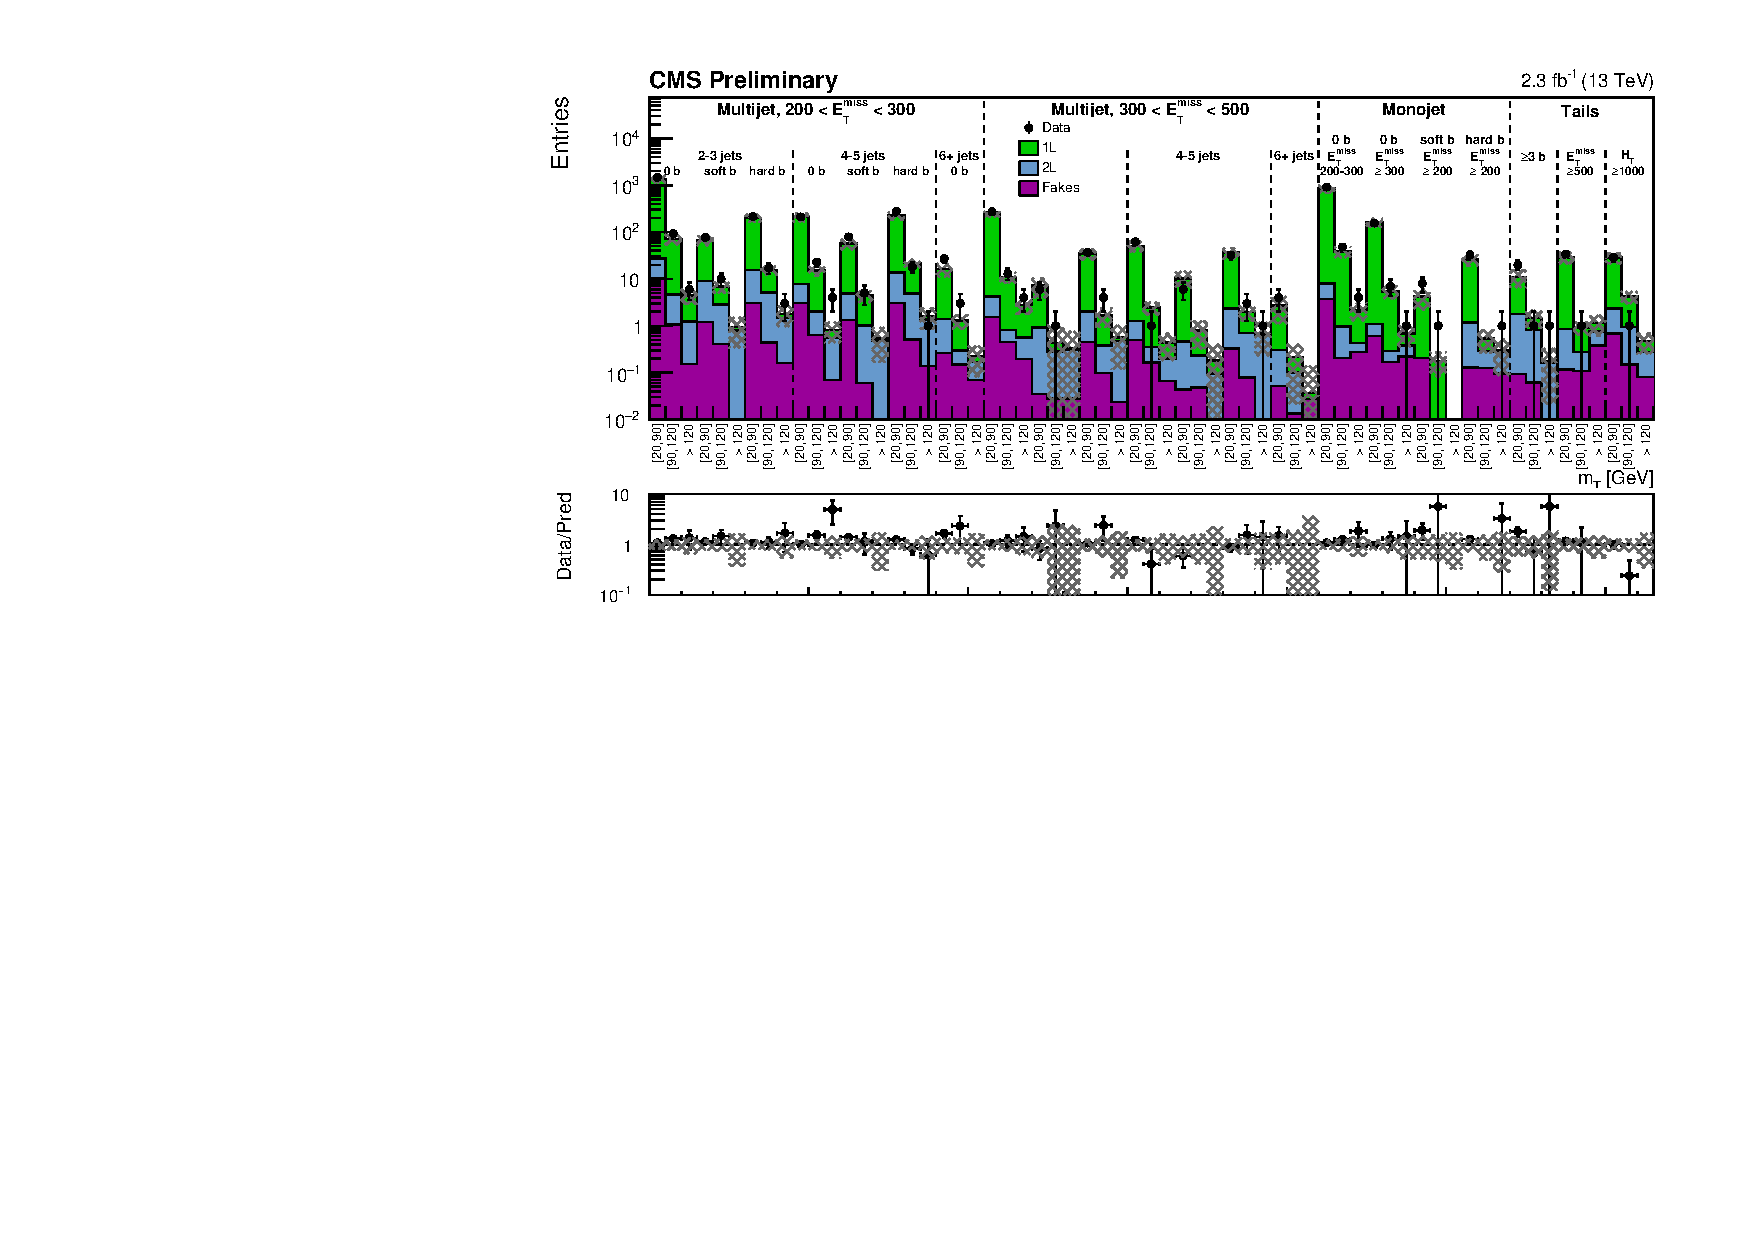
\includegraphics[width=0.95\textwidth]{soft/figs/c_DataVsPrediction_Syst_log}
	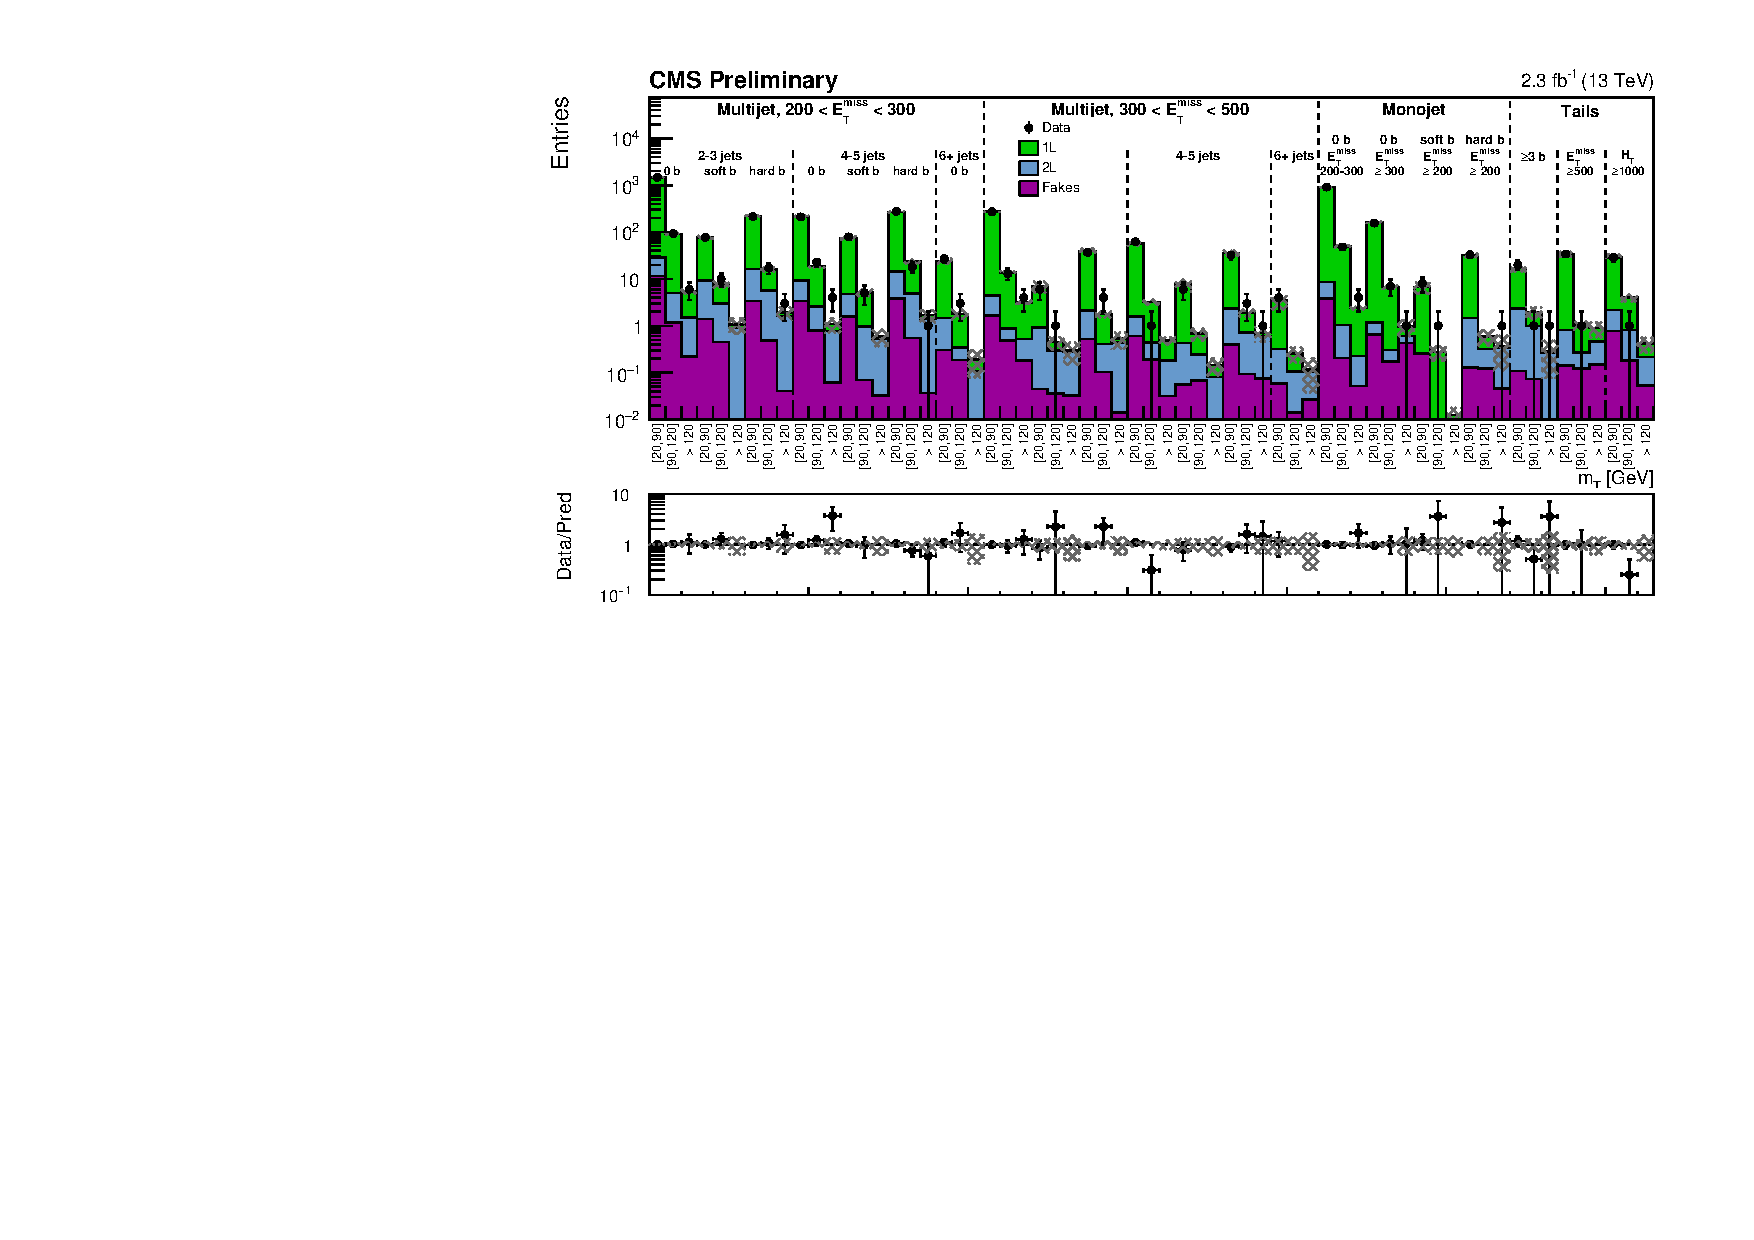
\includegraphics[width=0.95\textwidth]{soft/figs/c_DataVsPostFitEstimates_log}
	\caption{The predicted background yields compared to the observed number of events in data for pre-fit (top) and post-fit (bottom) background estimates. The \mt bins are shown on the $x$-axis, and the grey hatched band represents the total uncertainty on the background yields for the pre-fit background estimates and the fit uncertainty for the post-fit estimates.}
	\label{fig:softresults}
\end{figure}

Additional fits using a background+signal hypothesis are used to set upper limits on the production cross sections of some simplified SUSY models producing soft leptons. A summary of the uncertainties on the simulated signal yield can be found in table \ref{tbl:softsignalSyst}. The post-fit background yield based on these inputs is used to set 95\% confidence level exclusion limits as shown in figure \ref{fig:softlimits}.

\begin{table}
	\centering
	\caption{Typical values of the systematic uncertainties associated with the simplified SUSY model signal yield for each interpretation in this search.}
	\begin{tabular}{l|c}
\hline
Source & Typical values [\%]  \\
\hline
Integrated luminosity & 2.7  \\
Lepton efficiency & 10  \\
Jet energy scale & 5  \\
b tagging efficiency & 0--20  \\
ISR & 15--30  \\
Renormalization  and factorization scales & 5  \\
Limited size of MC samples & 1--70  \\
\hline
	\end{tabular}
	\label{tbl:softsignalSyst}
\end{table}
\begin{figure}
	\centering
	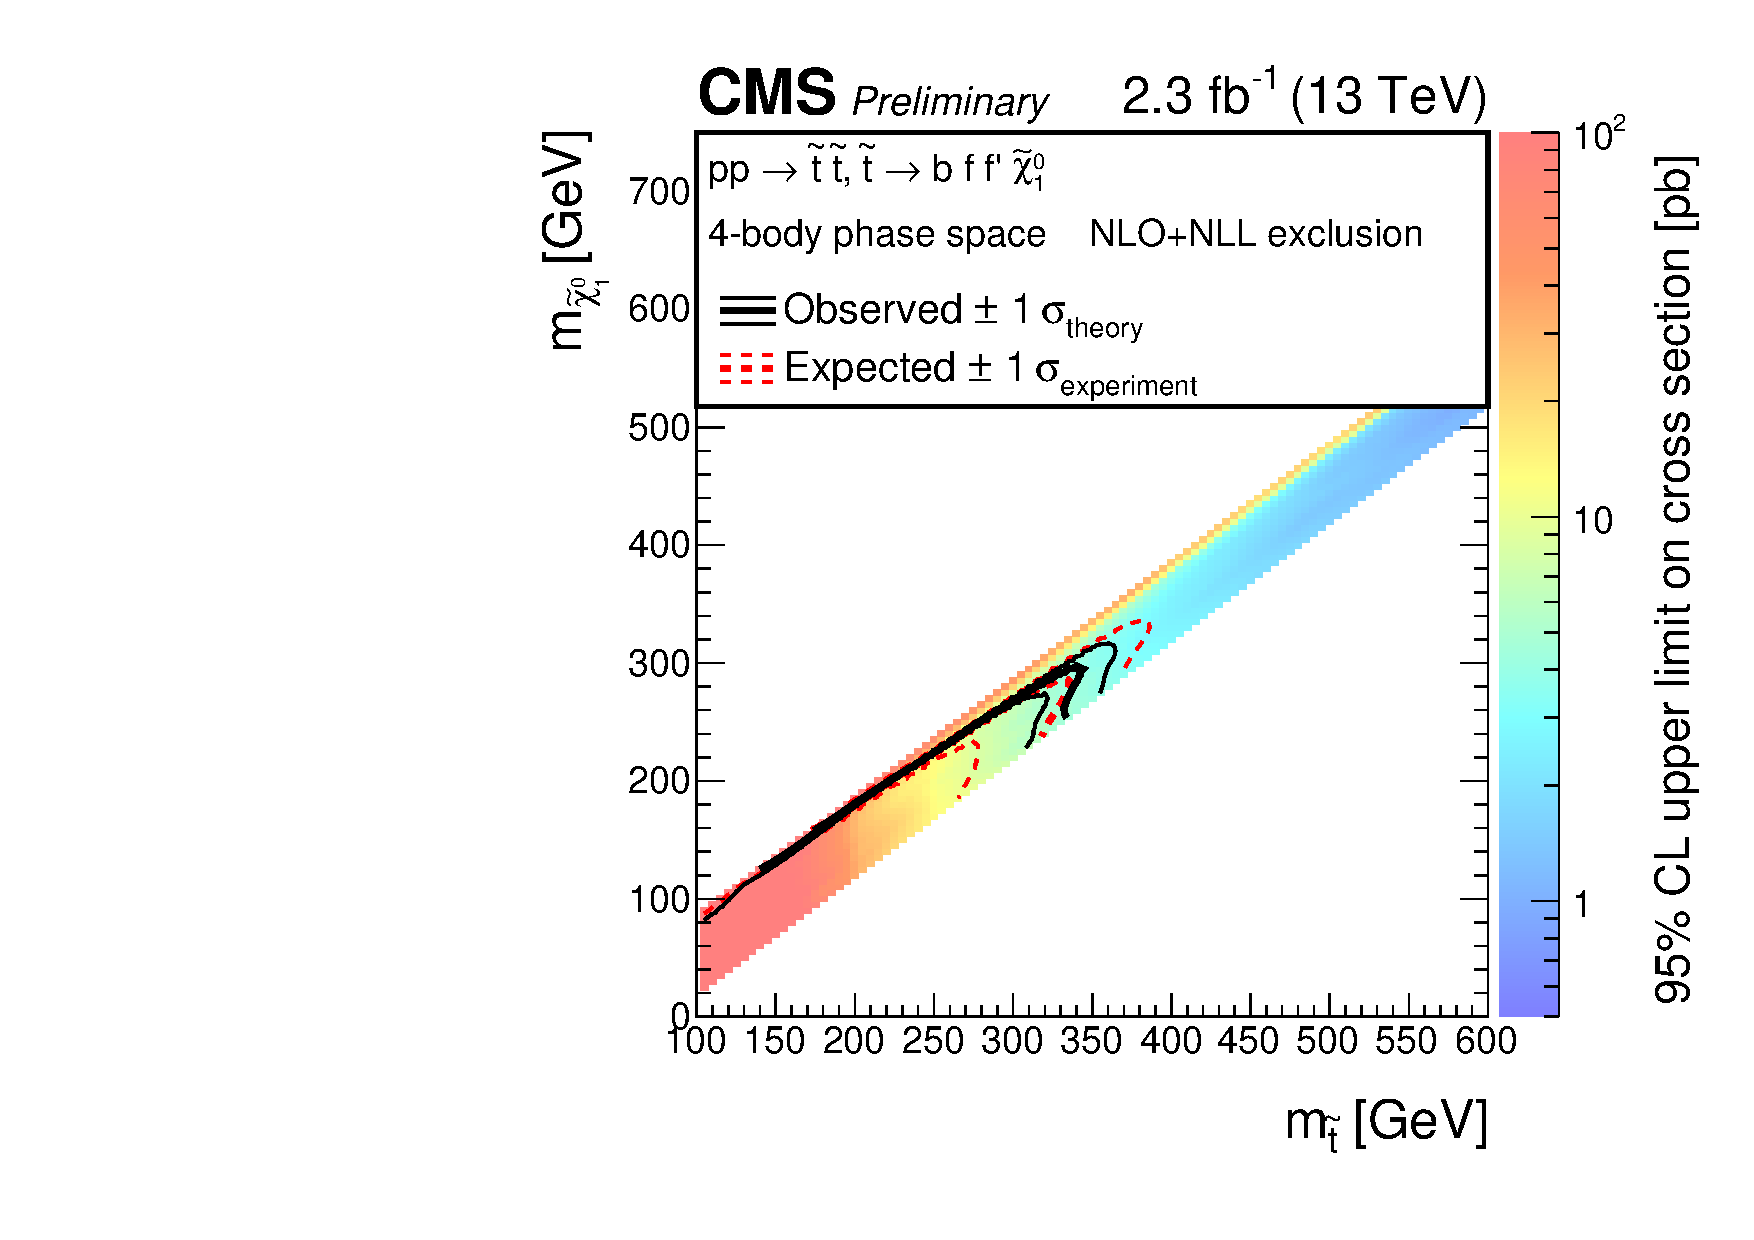
\includegraphics[width=0.45\textwidth]{soft/figs/T2-4bdXSEC}
	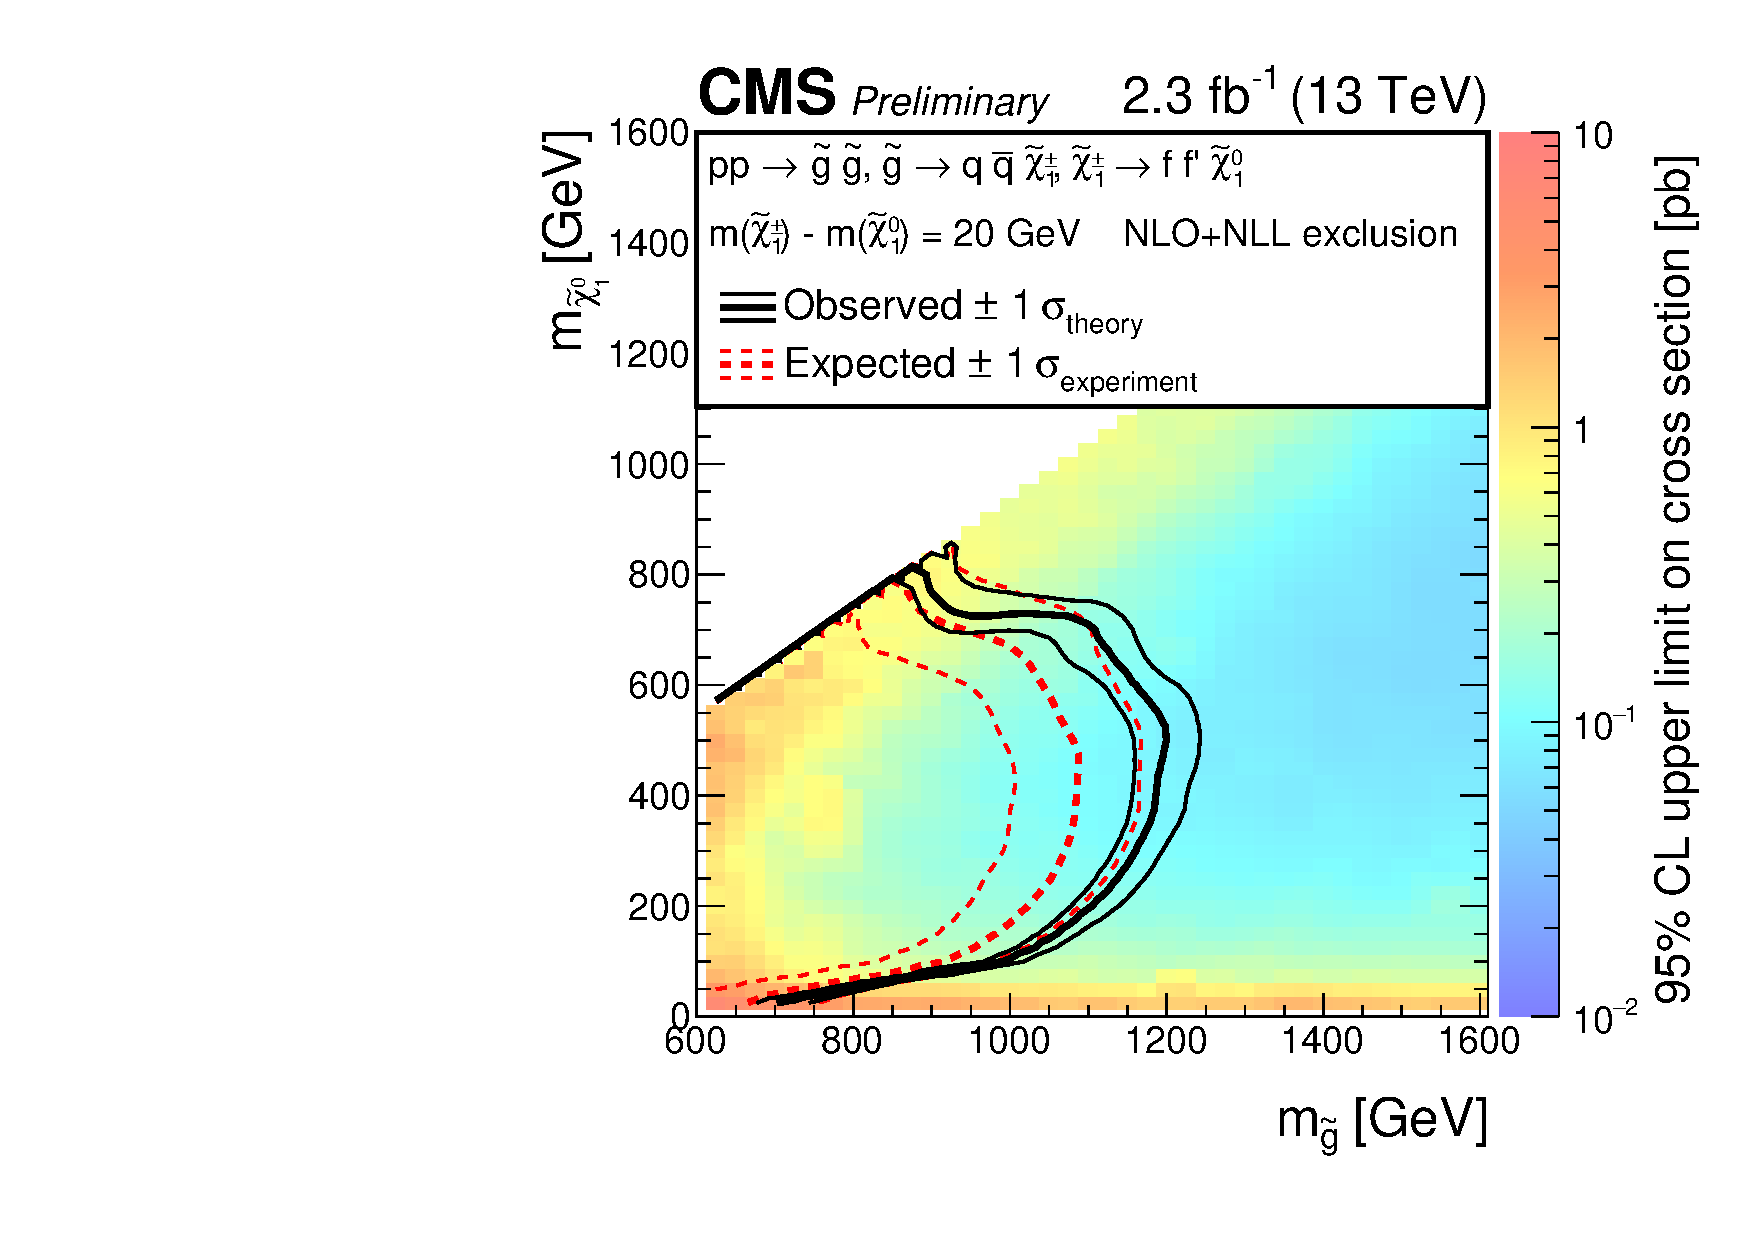
\includegraphics[width=0.45\textwidth]{soft/figs/T5qqqqWWXSEC}
	\caption{95\% confidence level exclusion limits for top squark (left) and gluino (right) production. Dashed red lines indicate the expected sensitivity and associated uncertainty, while black lines indicate the observed exclusion limit and its associated theoretical uncertainty based on the signal cross-section.}
	\label{fig:softlimits}
\end{figure}

\section{Future Extensions for an All-Hadronic Search}
\label{sec:future}

The extension of the all-hadronic analysis presented in this section illustrates one possible way to broaden the scope of an all-hadronic search to target additional sectors where new physics might reveal itself. However, there are similar analyses which may supersede the results of a naive single soft lepton search, and an additional question remains -- how much does the extension requiring a soft lepton outperform a traditional all-hadronic analysis? An all-hadronic search should have some discriminating power even against models which always generate soft leptons in the final state (since these leptons will occasionally be lost or mis-identified), and ironically may even have greatly discriminatory power than a soft lepton search when the leptons generated are ultra-soft (\pt $<<5\GeV$) and not reconstructed at all.

To benchmark the possible performance of an improved soft lepton analysis against an all-hadronic search, the performance of the \mttwo analysis on a squark production model generating soft leptons (T5qqWW) is compared to a soft lepton extension. With additional optimization of signal region binning -- in particular a finer binning in the low-\MET regime to target compressed spectra -- and assuming a typical background estimate uncertainty commensurate with previous analyses, it is possible for a soft lepton analysis to outperform an all-hadronic search as illustrated in figure \ref{fig:softfuture}. 
\begin{figure}
	\centering
	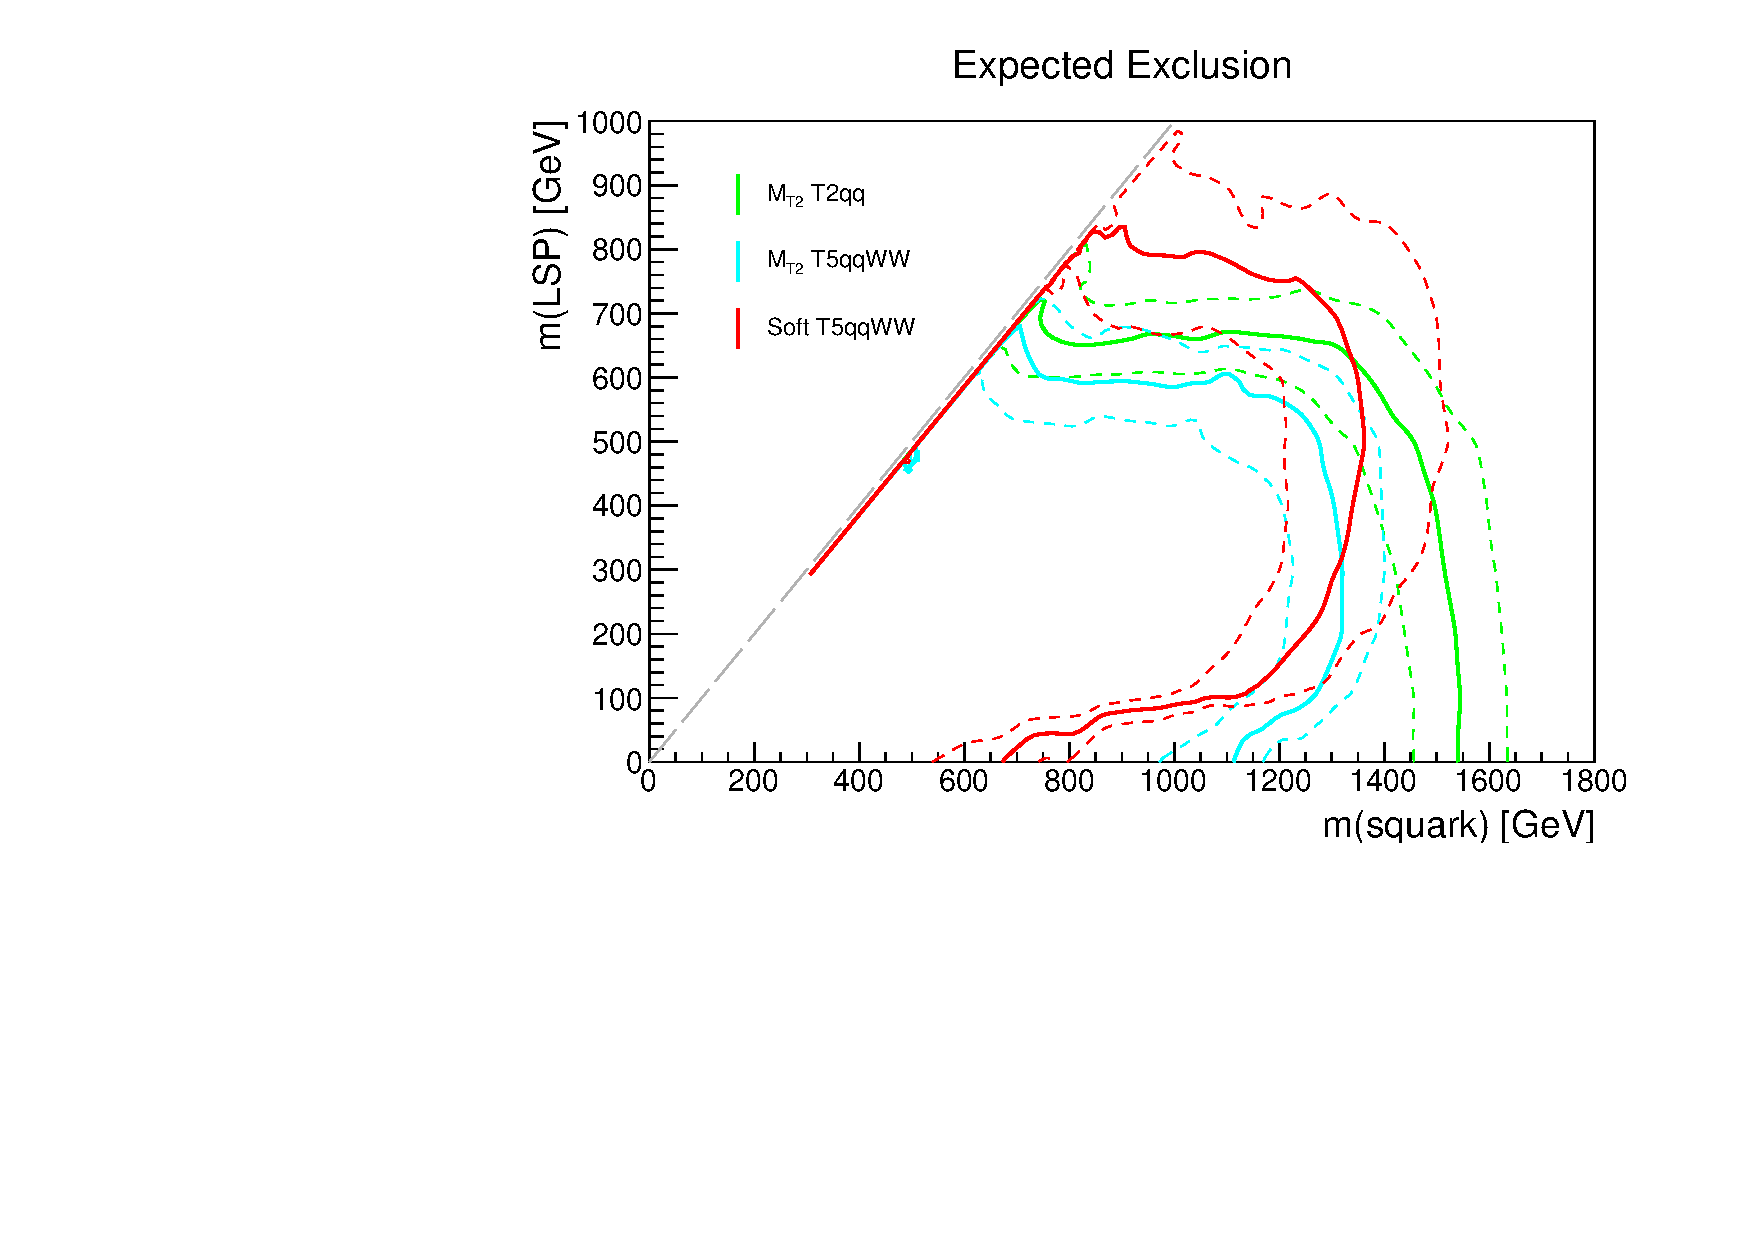
\includegraphics[width=0.75\textwidth]{soft/figs/expectedSoftLimit.pdf}
	\caption{The expected limits of the all-hadronic \mttwo analysis compared with a hypothetical soft lepton extension. The ``T2qq'' model is a typical squark production model as previously shown in figure \ref{fig:limitsSquark}, whereas the ``T5qqWW'' model is a similar squark production model where the squarks decay in a cascade including charginos, which radiate W bosons that may decay to soft leptons. While the performance of the \mttwo analysis in the hadronic model (green) is similar to the soft lepton model (blue), a soft lepton search can out-perform the all-hadronic equivalent near the diagonal where the mass splitting between the squarks and lightest supersymmetric particle is very small.}
	\label{fig:softfuture}
\end{figure}

Near the mass-diagonal where the parent particle mass (in this case, the squark) is very close to the LSP mass, the soft-lepton search can significantly outperform an all-hadronic equivalent, at the cost of performance in the light-LSP regime. The evidence suggests that a soft-lepton search could be used in conjunction with typical all-hadronic analyses to increase the total excluded phase space when targeting compressed models with nearly-degenerate mass splittings.

This work would not have been possible without all the members of the CMS collaboration, whose support made it possible to produce the figures and tables in this chapter.

% --------------------------------------------------------------------------- %
% --------------------------------------------------------------------------- %
